

\chapter{Приложение 1. Результаты экспериментов}


\def\figurename{Рис}
\begin{figure}[t]
	\centering
	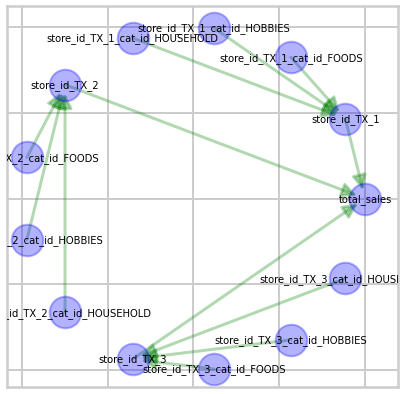
\includegraphics[width=0.5\columnwidth]{./img/fcm_lstm_map.png}
	\caption{Граф когнитивной карты для моделирования общего количества продаж с разбивкой по магазинам и категории товаров}
	\label{img:fcm_lstm_map}
\end{figure}


\begin{table}%
    \caption{Значения коэффициентов параметров ARIMAX(2, 0, 3)x(0, 1, 1, 7) с экзогенными переменными: индикатор дня недели и индикатор Рождества}
    \centering
    \begin{tabular}{|l|r||r|r|}
        \hline
            Параметр           &     Значение коэффициента  &  Дисперсия  &  P-value \\
        \hline
            intercept          &     3.7294                 &     1.686 &   0.027 \\
            Friday             &     0.0159                 &  2440.530 &   1.000 \\
            Monday             &     0.0045                 &  5202.932 &   1.000 \\
            Saturday           &    -0.0011                 &  7994.566 &   1.000 \\
            Sunday             &     0.0055                 &  4295.359 &   1.000 \\
            Thursday           &    -0.0069                 &  5951.614 &   1.000 \\
            Tuesday            &    -0.0007                 &  7381.431 &   1.000 \\
            Wednesday          &     0.0078                 &  3557.219 &   1.000 \\
            xmas               & -8738.4506                 &   399.352 &   0.000 \\
            ar.L1              &     0.0149                 &     0.067 &   0.824 \\
            ar.L2              &     0.8291                 &     0.056 &   0.000 \\
            ma.L1              &     0.3286                 &     0.074 &   0.000 \\
            ma.L2              &    -0.5438                 &     0.062 &   0.000 \\
            ma.L3              &    -0.1352                 &     0.038 &   0.000 \\
            ma.S.L7            &    -0.9363                 &     0.017 &   0.000 \\
            sigma2             &  1.264e+06                 &  3.87e+04 &   0.000 \\
        \hline
    \end{tabular}
    \label{tbl:arimax_coeffs_exogen}
\end{table}


% \end{figure}


% % \chapter{Основные правила форматирования}\label{app-format}

% %\addcontentsline{toc}{chapter}{}


% % Текст пояснительной записки должен готовиться для печати на листах формата А4, использоваться должен шрифт с засечками (Roman; обычно --- Times Roman или Times New Roman), 12 или 14 кегль. Размеры полей:

% % \begin{itemize}
% % 	\item верхнее: 20 мм.
% % 	\item нижнее: 20 мм.
% % 	\item левое: 10 мм.
% % 	\item правое: 25 мм.
% % \end{itemize}

% % Нумероваться должны все страницы, начиная с первой (титульной), однако сами номера следует проставлять на страницах, начиная со страницы реферата. Номер следует проставлять внизу страницу (в центре).

% % Заголовки оформляются тем же шрифтом, что и основной текст (т.е., соответственно, Times Roman или Times New Roman). Для заголовков первого уровня размер шрифта может быть больше размера шрифта основного текста (обычно 14-16).

% % Все разделы текста: реферат, оглавление, введение, три главы основного
% % содержания, список литературы, заключение, приложения --- должны снабжаться
% % содержательным заголовком и начинаться с новой страницы; сами заголовки следует
% % при этом центрировать (заголовки параграфов и пунктов выравниваются по ширине).
% % Следует обратить внимание, что заголовки всех разделов, кроме трех основных
% % глав, регламентированы; заголовки трех основных глав должны быть содержательными
% % и отражать суть соответствующей главы. Названия типа <<Аналитическая часть>> и <<Теоретическая глава>> --- \textit{недопустимы}.

% % Текст пояснительной записки может содержать рисунки и таблицы. Все рисунки и
% % таблицы должны снабжаться номерами и подписями:

% % \begin{itemize}

% % 	\item нумерация рисунков и таблиц должна быть сквозная (но раздельная, т.к. для рисунков своя, для таблиц --- своя);

% % 	\item в случае большого количества иллюстраций/таблиц, допускается <<вложенная>> нумерация (т.е. таблицу/рисунок можно снабжать составным номером в формате

% % 	$$\langle\mbox{номер главы}\rangle.\langle\mbox{номер внутри главы}\rangle;$$

% % 	\item подрисуночная подпись должна располагаться снизу по центру;

% % 	\item название таблицы следует помещать над таблицей слева, без абзацного
% % 	отступа в одну строку с ее номером через тире (ГОСТ 7.32-2001, п.6.6.1).

% % \end{itemize}

% % Здесь перечислены не все, а лишь основные требования к оформлению. Прочие
% % требования --- см. соответствующие ГОСТы.

% % Для того чтобы избежать больших отступов в списках, которые по умолчанию добавляют окружения \texttt{itemize} и \texttt{enumerate}, следует использовать
% % \texttt{compactitem} (для маркированных списков) и \texttt{compactenum} (для нумерованных списков) из пакета \texttt{paralist}.
% % Например:

% % \begin{compactitem}
% % 	\item это;
% % 	\item не нумерованный;
% % 	\item список;
% % 	\item без лишних промежутков.
% % \end{compactitem}

% % И для нумерованных списков:

% % \begin{compactenum}[1)]
% % 	\item нумерованные списки;
% % 	\item пакета \texttt{paralist};
% % 	\item еще и удобно настраивать;
% % 	\item (например, менять формат номера).
% % \end{compactenum}

% % \noindent или

% % \begin{compactenum}[a)]
% % 	\item это другой;
% % 	\item нумерованный;
% % 	\item список;
% % 	\item без лишних промежутков;
% % 	\item и с буквенной нумерацией.
% % \end{compactenum}

% % А если хочется нумерацию сделать ангоязычной, то нужно использовать окружение \texttt{other\-language} (таким образом: \verb|\begin{otherlanguage}[numerals=latin]{russian}|)

% % \setkeys{russian}{numerals=latin}
% % %\selectlanguage{russian}
% % %\begin{otherlanguage}[numerals=latin]{russian}
% % \begin{russian}
% % \begin{compactenum}[a)]
% % 	\item это другой;
% % 	\item нумерованный;
% % 	\item список;
% % 	\item без лишних промежутков;
% % 	\item и с буквенной нумерацией.
% % \end{compactenum}
% % \end{russian}
% % %\end{otherlanguage}

% % \textbf{Замечание.} По неизвестным причинам, переключения не происходит, хотя должно.